\section{架构范式}
沿着以表征为中心的世界模型观点，本节依据系统如何表示并推进世界状态，对现有系统进行分类。我们区分三类模型：直接在像素、体素或视频词元上预测的观测层模型，学习紧凑预测状态的潜在空间模型，以及引入显式空间、几何或实体层结构的三维增强模型（3D-enhanced model）或物体中心模型（object-centric model）。随后讨论跨范式统一的趋势，即在共享架构中整合生成、理解、交互，以及多模态（multimodal）信息与物理世界的关联。表\ref{tab:wm_architecture_comparison}概括了主要取舍与代表系统。

\subsection{观测层生成式世界模型}
观测层生成式世界模型将世界建模视为高维观测合成，直接预测未来像素、体素或视频词元。近期的大规模视频生成器，包括Sora类模型\citep{openai2024sora}、Wan\citep{wan2025wan}、Happy Horse\citep{happyhorse2026}、Seedance系列\citep{gao2025seedance,seedance2026seedance2}、Movie Gen\citep{polyak2024moviegen}、HunyuanVideo\citep{kong2024hunyuanvideo}、CogVideoX\citep{yang2024cogvideox}和Kling系列\citep{kling2025omni}，并不都属于严格的决策中心意义上的世界模型，但代表了从大规模视频学习物理先验的观测层路线。更明确具有交互能力的系统，包括Genie系列\citep{bruce2024genie,parkerholder2024genie2,genie3}、GameNGen\citep{valevski2025gamengen}、DIAMOND\citep{alonso2024diamond}和Oasis\citep{decart2024oasis}，则从被动续接视频迈向可控的环境生成。在物理与驾驶场景中，Cosmos\citep{nvidia2025cosmos}、GAIA-1\citep{hu2023gaia1}、DriveDreamer\citep{wang2023drivedreamer}、Drive-WM\citep{wang2023drivewm}以及Waymo World Model\citep{waymo2026worldmodel}进一步将观测层生成用于以轨迹、行动或场景为条件的模拟。

其主要优势在于规模：互联网视频提供了庞大的弱监督语料，可用于学习外观、运动、物体交互和场景动力学。因此，这些模型往往具有较高的视觉保真度，且覆盖广泛的现实世界现象。然而，视觉可信并不等于物理正确。像素空间模型生成的推演可能局部可信、整体却不一致；特别是在长时域中，物体恒存性、接触动力学、因果性或场景一致性方面的错误会逐渐积累。它们的计算成本也很高，因为预测发生在高维观测空间。因此，Diffusion Forcing\citep{chen2024diffusionforcing}、VideoPoet\citep{kondratyuk2024videopoet}、Wan\citep{wan2025wan}和Cosmos\citep{nvidia2025cosmos}等系统，探索如何把大型生成式视频模型的感知优势扩展到时间连贯的序列级预测。因此，评估观测层世界模型的核心标准不仅是感知保真度，还包括：在行动、指令、轨迹或其他条件信号下，所生成轨迹能否保持物理一致、因果连贯和可控。

\begin{table*}[t]
\centering
\setlength{\tabcolsep}{3pt}
\renewcommand{\arraystretch}{1.08}
\caption{主要世界模型架构范式的优势与局限。}
\label{tab:wm_architecture_comparison}
\vspace{.2cm}
\resizebox{\linewidth}{!}{
\begin{tabular}{@{} c | c | c | c @{}}
\hline
\textbf{范式} & \textbf{优势} & \textbf{局限} & \textbf{代表系统} \\
\hline
\makecell{观测层} &
\makecell{视觉保真度高；\\
输出直观；\\
可随互联网视频扩展} &
\makecell{生成成本高；\\
物理不一致；\\
长时域推演漂移} &
\makecell{\citep{openai2024sora}\\
\citep{bruce2024genie}\\
\citep{wan2025wan}\\
\citep{gao2025seedance}\\
\citep{nvidia2025cosmos}\\
\citep{chen2024diffusionforcing}} \\
\hline
\makecell{潜在空间} &
\makecell{高效想象式规划；\\
紧凑潜在状态；\\
适合扩展至长时域} &
\makecell{丢失关键细节；\\
难以目视检查；\\
目标不匹配} &
\makecell{\citep{ha2018worldmodels}\\
\citep{hafner2019planet}\\
\citep{hafner2019dreamer}\\
\citep{hafner2021dreamerv2}\\
\citep{hafner2023dreamerv3}\\
\citep{hansen2023tdmpc2}\\
\citep{schrittwieser2020muzero}\\
\citep{assran2023ijepa}\\
\citep{bardes2024vjepa}}\\
\hline
\makecell{三维／物体中心} &
\makecell{空间一致性更好；\\
物体级推理；\\
处理视角与遮挡} &
\makecell{需要结构化监督；\\
难以处理动态场景} &
\makecell{\citep{zheng2024occworld}\\
\citep{zhang2025robooccworld}\\
\citep{mildenhall2020nerf}\\
\citep{kerbl20233dgaussians}\\
\citep{worldlabs2025marble}\\
\citep{wu2023slotformer}\\
\citep{huang2025enerverse}} \\
\hline
\makecell{跨范式\\统一} &
\makecell{结合生成、\\理解、交互\\及多模态与物理世界的关联} &
\makecell{尚处早期；\\
模态对应关系问题；\\
行动保真度；\\
评估尚无定论} &
\makecell{\citep{liu2025lwm}\\
\citep{ge2024worldgpt}\\
\citep{zhou2025hermes}\\
\citep{ye2026dreamzero}\\
\citep{zhu2025uwm}\\
\citep{nvidia2026cosmos3}} \\
\hline
\end{tabular}}
\end{table*}

\subsection{潜在空间世界模型}
从像素空间转向潜在空间世界模型，不仅是效率提升，也反映了从视觉外观建模向任务相关状态演化建模的根本转变。PlaNet\citep{hafner2019planet}和Dreamer家族\citep{hafner2019dreamer,hafner2021dreamerv2,hafner2023dreamerv3}等早期潜在世界模型，利用循环状态空间模型（recurrent state-space model，RSSM）等潜在动力学模型，将高维观测编码为紧凑状态，并高效进行基于想象的规划。由于推演的是紧凑潜在状态，而非全分辨率像素，这些方法更容易扩展到长时域，更好地处理部分可观测性，也允许智能体在固定计算预算下评估更多假想未来。

除了效率之外，潜在建模还改变了世界建模的优化目标。潜在空间模型不必耗费容量重建每一处RGB细节，而可以聚焦于变化较慢、与决策相关、决定未来可控性的因素，如几何、物体关系、可供性（affordance）、接触动力学和时间演化。TD-MPC与TD-MPC2等基于模型的控制方法\citep{hansen2022tdmpc,hansen2023tdmpc2}进一步表明，规划可以直接在学习得到的、面向任务的潜在空间中进行，无需完整像素解码器即可高效优化轨迹。类似地，对比式及无重建世界模型\citep{kipf2019cswm,okada2022dreamingv2,poudel2023recore}表明，避免像素级重建，可以减轻对纹理、光照和细小光度变化等高频外观干扰因素的过拟合，从而提高鲁棒性。JEPA类预测表征学习等较新方法\citep{assran2023ijepa,bardes2024vjepa,assran2025vjepa2}通过预测表征而非像素，进一步质疑完整视觉重建的必要性。更广泛地，LDA-1B\citep{lyu2026lda1b}和Motus\citep{bi2025motus}等具身学习系统表明，有效策略往往可以从紧凑、面向任务的潜在表征中学得，而不必逼真重建整个视觉场景。从这个意义上说，潜在世界模型不仅可能更快，也可能更适合控制：保留低频、具有因果相关性的结构，同时抑制表面视觉细节，可以支持更鲁棒、更准确的决策。

不过，主要风险是过度抽象会丢弃视觉上很小、对决策却至关重要的信息，如夹爪与物体的接触、细小障碍物、微妙的物体姿态变化或形变。因此，核心挑战不只是压缩观测，而是学习一种潜在表征：舍弃外观噪声，同时保留决定未来可控性的因素。这也改变了评估方式：不能只按重建误差或预测误差评价潜在世界模型，还应检验其推演是否保留下游规划与控制所需的信息。

\subsection{三维增强与以物体为中心的世界模型}
三维增强和以物体为中心的世界模型，推动世界建模从单纯的帧预测转向结构化场景理解。传统视频模型可能生成视觉上可信的未来帧，但内部状态常难以解释，也可能不对应场景真实的三维布局。对具身人工智能而言，这构成了限制：模型还应支持对自由空间、物体位置、遮挡、视角变化、物体恒存性和物理合理性的推理。因此，近期研究探索了三维占据（3D occupancy）、鸟瞰图（bird's-eye view，BEV）表征、类似NeRF的辐射场（radiance field）、三维高斯泼溅，以及物体槽位（object slot），作为世界模型中结构更明确的状态空间\citep{mildenhall2020nerf,kerbl20233dgaussians,locatello2020slotattention,wu2023slotformer,zheng2024occworld,zhang2024bevworld,zhang2025robooccworld}。

一个方向是基于占据与BEV的世界建模。这些表征比像素更直接地揭示场景空间结构，因此有利于推理自由空间、障碍物、语义区域和未来场景演化。在自动驾驶中，OccWorld、OccSora、Drive-OccWorld和BEVWorld等系统，在占据或类似BEV的空间中学习未来场景动力学\citep{zheng2024occworld,wang2024occsora,yang2024driveoccworld,zhang2024bevworld}。在机器人学中，RoboOccWorld依据空间观测历史和未来相机姿态预测三维语义占据，将这种结构化状态观点扩展到室内具身预测\citep{zhang2025robooccworld}。这一家族的主要优势，是预测结果可以按空间位置查询，而不只是视觉上可信。

另一类方法使用连续或基于点的三维场景表征。NeRF和三维高斯泼溅提供具有几何信息的状态，支持新视角渲染与更强的视角一致性\citep{mildenhall2020nerf,kerbl20233dgaussians}。Marble、RenderWorld、GaussianWorld和GWM等近期系统，将这一思想扩展到持久三维世界生成、驾驶世界建模、流式占据预测及机器人操作\citep{worldlabs2025marble,yan2024renderworld,zuo2025gaussianworld,lu2025gwm}。与纯视频生成相比，这些模型能更好地跨视角、跨时间保留空间结构，但在动态场景和长时域交互方面仍面临困难。

以物体为中心的世界模型解决一个互补的问题：即使稠密的三维状态，也未必能分离出重要实体。OP3、C-SWM、Slot Attention、SAVi和SlotFormer等方法，学习物体或槽位层的表征与动力学，支持组合性更强的预测和推理\citep{veerapaneni2019op3,kipf2019contrastive,locatello2020slotattention,kipf2022savi,wu2023slotformer}。FOCUS和Object-Centric World Model for Language-Guided Manipulation等近期机器人系统，进一步将物体层抽象连接到操作及指令条件预测\citep{ferraro2023focus,jeong2025objectcentricwm}。这种抽象很有用，因为许多具身任务自然地围绕持续存在的实体及其关系定义，而非全局图像模式。

最有前景的方向，是结合这些表征，而非将其视为相互竞争的选择。占据表征支持自由空间与碰撞推理，NeRF和三维高斯表征支持视角一致的渲染，物体槽位则支持组合推理。EnerVerse和EnerVerse-AC等混合具身系统，通过连接多视角预测、记忆、四维场景表征、指令或行动条件化，以及具身未来生成，已经指向这一方向\citep{huang2025enerverse,jiang2025enerverseac}。更普遍的启示是，未来具身世界模型可能需要在共享物理表征中结合空间几何、时间记忆、物体结构及与交互的关联。

同时，加入三维结构并不会自动解决世界建模问题。模型可能准确重建空间，却仍无法捕捉可供性、因果性、物体恒存性或任务相关语义。物体中心模型紧凑且可解释，但在杂乱场景和遮挡下可靠地发现物体，仍然困难。NeRF或三维高斯模型可以渲染精细视图，但扩展到动态场景、长时域预测和闭环交互仍有挑战。因此，关键问题不是世界模型看起来是否更加三维，而是其状态是否构成对物理世界有用且连贯的表征。强大的具身世界模型，应具有几何一致性、时间上的持续一致性、物体感知能力和物理合理性，并能供下游推理、规划或控制模块使用。

\subsection{统一趋势：全模态世界模型}
\begin{figure}[t]
    \centering
    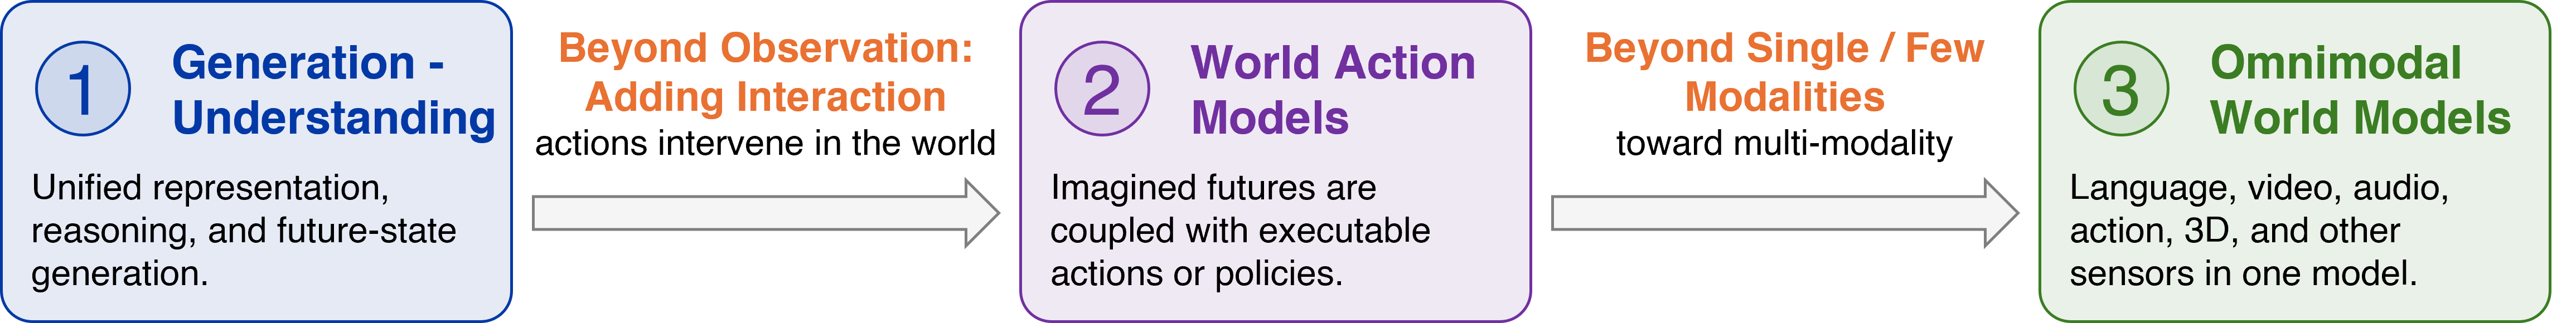
\includegraphics[width=\linewidth]{figs/omnimodal.png}
    \caption{世界模型架构的统一趋势。生成与理解统一模型首先通过引入交互及与行动的关联，超越被动观测，形成世界行动模型（WAM）。此后，该范式进一步超越单模态或少数模态建模，迈向全模态模型，在共享物理表征中整合语言、视频、音频、行动、三维结构及其他传感器信号。}
    \label{fig:omnimodal_world_model_trend}
\end{figure}

世界模型研究中逐渐形成一种共识：未来世界模型不应是纯生成器，而应是生成与理解统一的模型。世界模型不仅应合成未来观测，还应理解物体、空间关系、时间动力学、因果性和物理合理性。LWM\citep{liu2025lwm}、WorldGPT\citep{ge2024worldgpt}、HERMES\citep{zhou2025hermes}、HERMES++\citep{zhou2026hermespp}、GaussianDWM\citep{deng2026gaussiandwm}和UniDrive-WM\citep{xiong2026unidrivewm}等系统，更明确地体现了这一方向，尝试在统一框架中连接场景或视频理解与未来状态生成。相邻领域的多模态基础模型，如Chameleon\citep{chameleon2025}、Janus／Janus-Pr\citep{wu2024janus,chen2025januspro}和Emu系列\citep{wang2024emu3,cui2025emu35}，进一步表明理解与生成可以在共享的词元化或自回归架构中处理，为这一趋势提供支持。综合来看，世界建模正在超越视觉上吸引人的合成，迈向对动态世界联合进行表示、推理与生成的架构。

然而，物理世界不仅被观测，也承受行动。从部分可观测决策的角度看，具身智能体只能接收底层世界状态的部分观测，而其行动会干预潜在状态转移，塑造未来观测，如图\ref{fig:omnimodal_world_model_trend}所示。因此，仅统一生成与理解还不够。用于物理人工智能的世界模型，不仅应表征并生成未来状态，还应将想象的未来连接到可执行行动。这推动了世界行动模型（WAM）的出现\citep{wang2026wam_survey}，它们在共享生成框架中整合世界建模与行动或策略建模。WAM不再把动力学预测和策略学习作为独立模块，而是直接从视频—行动数据学习二者的耦合。例如，DreamZero\citep{ye2026dreamzero}表明，联合建模视频和行动，可以把世界模型转化为零样本策略；LingBot-VA\citep{li2026lingbotva}在自回归视频—行动框架中统一视觉动力学预测与行动推断；$\tau$0-WM\citep{zhou2026tau0wm}则为机器人操作整合行动生成、视频预测及未来状态评估。UWM\citep{zhu2025uwm}、Cosmos Policy\citep{kim2026cosmospolicy}、GigaWorld-Policy\citep{ye2026gigaworldpolicy}、Fast-WAM\citep{yuan2026fastwam}和Flash-WAM\citep{akbari2026flashwam}等相关系统，进一步探索视频预测与行动生成的不同耦合方式，包括联合扩散、以行动为中心的预测，以及无需在测试时显式想象视频的更快推理。这些模型共同标志着：研究正从被动世界模拟，转向既能想象物理未来，又能生成以这些未来为依据的行动的生成模型。

此外，世界模型正从单模态或少数模态场景扩展至全模态物理建模，在共享物理世界表征中整合语言、图像、视频、音频、行动、三维结构和传感器数据，见图\ref{fig:omnimodal_world_model_trend}。NVIDIA Cosmos 3\citep{nvidia2026cosmos3}是这一更广泛尝试的鲜明代表：它明确希望在混合Transformer架构中统一语言、图像、视频、音频和行动，从以视觉为中心的生成迈向通用物理人工智能后端。其他近期系统虽尚非完整全模态世界模型，也为这一方向提供了重要组成部分。Seedance 2.0\citep{seedance2026seedance2}探索以文本、图像、音频和视频为输入的统一多模态音视频生成；Wan／Wan2.1\citep{wan2025wan}提供可扩展的开放视频生成骨干；腾讯HunyuanVideo与HunyuanWorld系列\citep{kong2024hunyuanvideo,hunyuanworld2025}将视频生成扩展至可探索、可交互的三维世界构建；Kling-Omni\citep{kling2025omni}整合多模态指令遵循、视频生成、编辑与推理；Qwen-Omni\citep{qwen2025omni}则展示了如何在统一全模态基础模型中处理语言、视觉、音频和视频。综合来看，生成、理解、交互、空间推理和多模态物理预测，正在汇入共享的模型骨干。从这个意义上说，这一统一趋势源于物理人工智能的需求：用一个模型理解当下、想象合理未来、与世界交互，并整合多模态物理信号。
